\documentclass[a4paper]{article}

\usepackage[a4paper,top=2cm,bottom=2cm,left=0.5cm,right=0.5cm,marginparwidth=1.75cm]{geometry}
\usepackage[utf8]{inputenc}
\usepackage[english, russian]{babel}
\usepackage[]{amsmath,amsfonts,amssymb,amsthm,mathtools}
\usepackage[]{wasysym}
\usepackage[]{float}
\usepackage{multicol}
\usepackage{amsfonts}
\usepackage{indentfirst}
\usepackage{longtable}
\usepackage{natbib}
\usepackage{mathrsfs}
\usepackage{wrapfig}
\usepackage{graphicx}
\usepackage{mathtext}
\usepackage{amsmath}
\usepackage{siunitx} % Required for alignment
\usepackage{subfigure}
\usepackage{multirow}
\usepackage{rotating}
\usepackage[T1,T2A]{fontenc}
\usepackage{caption}
\usepackage{gensymb}

\date{\today}
\title{Лабораторная работа 3.4.5}
\author{Сидорчук Максим, Б01-204}

\begin{document}
\maketitle
\paragraph*{Цель работы:} изучение петель гистерезиса ферромагнитных материалов с помощью осциллографа.

\paragraph*{Оборудование:} автотрансформатор, понижающий трансформатор, амперметр и вольтметр (мультиметры), резистор, делитель напряжения, интегрирующая
цепочка, электронный осциллогра, тороидальные образцы с двумя обмотками..

\section{Теоретическое введение}

\begin{wrapfigure}{l}{0.6\textwidth}
	\vspace{-20pt}
	\begin{center}
		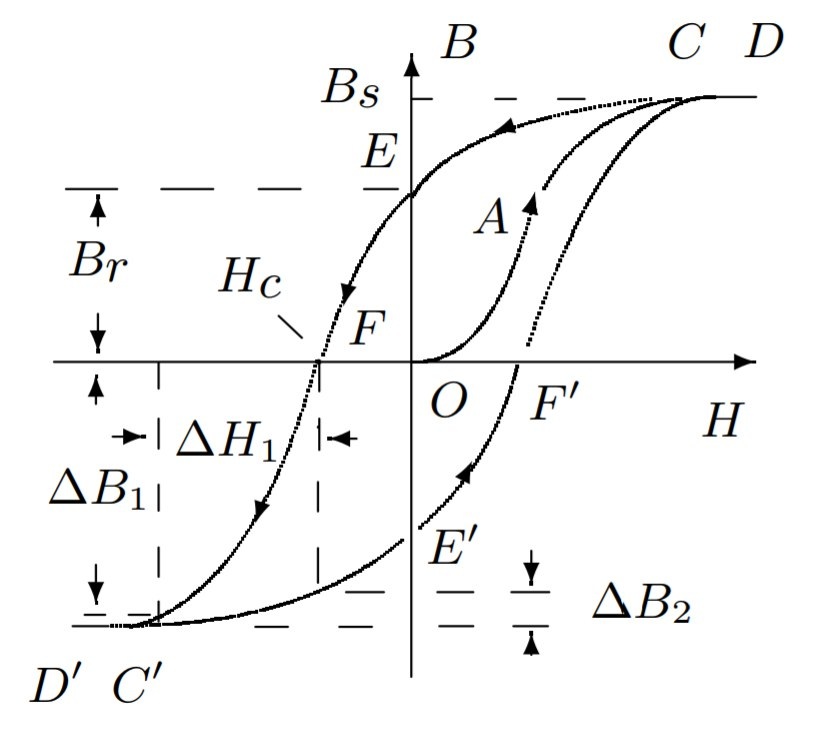
\includegraphics[width=0.7\linewidth]{gist3.jpg}
		\label{fig:sdfsafd}
	\end{center}
	\vspace{-10pt}
	\caption{Петля гистерезиса ферромагнетика}
\end{wrapfigure}

Магнитная индукция $\vec{B}$ и напряженность магнитного поля
$\vec{H}$ в ферромагнитном материале неоднозначно связаны
между собой: индукция зависит не только от напряженности, но
и от предыстории образца. Связь между индукцией
и напряженностью поля типичного ферромагнетика иллюстрирует рис. 1. Если
к размагниченному образцу начинают прикладывать магнитное поле, то его намагничивание следует кривой $ OACD $, выходящей
из начала
координат. Эту кривую называют \textit{основной кривой намагничивания}.


Индукция $\vec{B}$ в образце состоит из индукции, связанной с намагничивающим полем
$\vec{B}$, и индукции, создаваемой самим намагниченным
образцом.
В системе СИ эта связь имеет вид

$$\vec{B} = \mu_{0}(\vec{H}+\vec{M}),$$

где $\vec{M}$- \textit{намагниченность} - магнитный момент единичного объема образца, а $\mu_{0}$ - магнитная постоянная.

Намагнитим образец до насыщения - до точки D. Соответствующее
значение индукции $B_{s}$ называют индукцией насыщения. При уменьшении поля $H$ до нуля зависимость $B(H)$ имеет вид кривой $DCE$, и при нулевом поле индукция имеет конечное ненулевое значение. Это остаточная индукция $B_{r}$ . Чтобы размагнитить образец, то есть перевести его в состояние
$F$, необходимо приложить "обратное" магнитное
поле $H_{c}$, которое называют коэрцитивной силой.

Замкнутая кривая $DEFD'E'F'D$, возникающая при циклическом
перемагничивании образца, намагниченного до насыщения, называется \textit{предельной петлей гистерезиса.}


\subsection{Измерение магнитной индукции в образцах.}
Магнитную индукцию удобно определять с помощью ЭДС, возникающей при изменении магнитного потока Ф в катушке, намотанной на образец:

$$\mathscr{E} = -\dfrac{dФ}{dt}.$$

Тогда отсюда и из формулы $Ф=BSN_{и}$ получаем:
$$|B|=\dfrac{1}{SN_{и}}\int \mathscr{E}dt.$$
Для интегрирования сигнала применяют интегрирующие схемы (рис. 2).

\begin{wrapfigure}{l}{0.6\textwidth}
	\vspace{-20pt}
	\begin{center}
		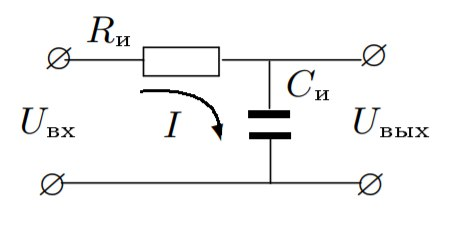
\includegraphics[width=0.7\linewidth]{gist2.jpg}
		\label{fig:sdfsafd}
	\end{center}
	\vspace{-10pt}
	\caption{Интегрирующая RC-цепь}
\end{wrapfigure}

Если выходной сигнал намного меньше входного ($U_{вых}\ll U_{вх},$) ток в цепи пропорционален входному напряжению: $I\simeq\dfrac{U_{вх}}{R}$, а напряжение на емкости С

$$U_{вых}\simeq\dfrac{1}{RС}\int U_{вх}dt.$$

Этот вывод тем ближе к истине, чем больше постоянная $\tau=RC$ превосходит характерное время процесса (например, его период). Для синусоидальных напряжений

$$U_{вых}=\dfrac{U_{вх}}{RC\Omega},$$

где $\Omega$ - частота сигнала.

В итоге, обозначив параметры интегрирующей цепи через $R_{и}$ и $C_{и}$, получаем

$$ |B|=\dfrac{1}{SN_{и}}\int U_{вх}dt=\dfrac{R_{и}С_{и}}{SN_{и}}U_{вых}.$$

\section{Экспериментальная установка.}
Схема экспериментальной установки показана на рис. 3.

Действующее значение переменного тока в обмотке N0 измеряется амперметром А (мультиметром GDM). Последовательно с амперметром включено сопротивление $R_{0}$, напряжение с которого подается на вход X электронного осциллографа (ЭО). Это напряжение пропорционально току в обмотке $N_{0}$, а следовательно и напряженности H магнитного поля в образце.

Для измерения магнитной индукции B с измерительной обмотки $N_{И}$ на вход интегрирующей RC -цепочки подается напряжение $U_{И}$ (UВХ), пропорциональное производной $\dot{B}$, а с выхода снимается напряжение $U_{C}$($U_{ВЫХ}$), пропорциональное
величине B , и подается на вход Y осциллограа.
Замкнутая кривая, возникающая на экране, воспроизводит в некотором масштабе (различном для осей X и Y ) петлю гистерезиса. Чтобы придать этой кривой количественный смысл, необходимо установить масштабы изображения, т.е. провести калибровку каналов X и Y ЭО. Для этого, во-первых, надо узнать, каким напряжениям (или токам) соответствуют амплитуды сигналов, видимых на экране, и во-вторых,  каким значениям B и H соответствуют эти напряжения
(или токи).

\begin{figure}[H]
	\centering
	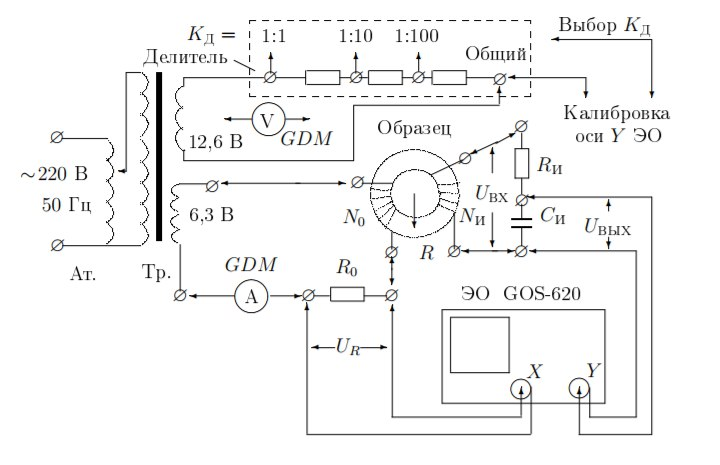
\includegraphics[width=\linewidth]{gist.jpg}
	\caption{Схема установки для исследования намагничивания образцов}
	\label{fig:Holl2}
\end{figure}


\section{Ход работы}

\begin{enumerate}
	\item Запишем данные установки:

	      $R_{0}=0.3$ Ом \\
	      $R_\text{и}=20$ кОм \\
	      $C_\text{и}=20$ мкФ \\

	      Параметры тороидальных образцов:

	      \begin{itemize}

		      \item	\textbf{Пермаллой $ Fe-Ni $  НП50}:
		            $N_{0}=40$ витков;
		            $N_{и}=200$ витков;
		            $S=3.8 \text{см}^{2}$;
		            $2\pi R = 24 $ см.

		      \item	\textbf{Феррит 1000нн}:
		            $N_{0}=35$ витков;
		            $N_{и}=400$ витков;
		            $S=3.0 см^{2}$;
		            $2\pi R = 25 см $.

		      \item 	\textbf{Кремниевое железо $ Fe-Si $}:
		            $N_{0}=35$ витков;
		            $N_{и}=350$ витков;
		            $S=1.2 \text{см}^2$;
		            $2\pi R = 10$ см.
	      \end{itemize}


	\item Соберем схему (рис. 3) и настроим оборудование.

	\item Для каждого образца сфотографируем предельную петлю. Запишем значения коэффициентов усиления $K_{x}$ и $K_{y}$, ток $I_{эф}$. Измерим двойные амплитуды для коэрцитивной силы $2x(c)$ и индукции насыщения $2y(s)$. Результаты таковы:

	      \begin{itemize}

		      \item 	\textbf{Пермаллой}:

		            $K_{x}=4 \dfrac{\text{мВ}}{\text{дел}},$
		            $K_{y}=20 \dfrac{\text{мВ}}{\text{дел}},$
		            $I_\text{эф} = 228$ мА.
		            При этом $ 2x = 28$ дел, $2y = 16$ дел.

		      \item 	 \textbf{Феррит}:

		            $K_{x}=2 \dfrac{\text{мВ}}{\text{дел}},$
		            $K_{y}=2 \dfrac{\text{мВ}}{\text{дел}},$
		            $I_\text{эф} = 112$ мА.
		            При этом $ 2x = 18$ дел, $2y = 20$ дел.

		      \item 	\textbf{Кремниевое железо}:

		            $K_{x}=10 \dfrac{\text{мВ}}{\text{дел}},$
		            $K_{y}=10 \dfrac{\text{мВ}}{\text{дел}},$
		            $I_\text{эф} = 573$ мА.
		            При этом $ 2x = 40$ дел, $2y = 28$ дел.

	      \end{itemize}



	\item Снимем для каждого образца начальную кривую намагничивания (табл. 1-3), плавно уменьшая ток до нуля и отмечая вершины частных петель. По этим данным построим эти кривые (рис. 4-6).

		      \begin{figure}[H]
			      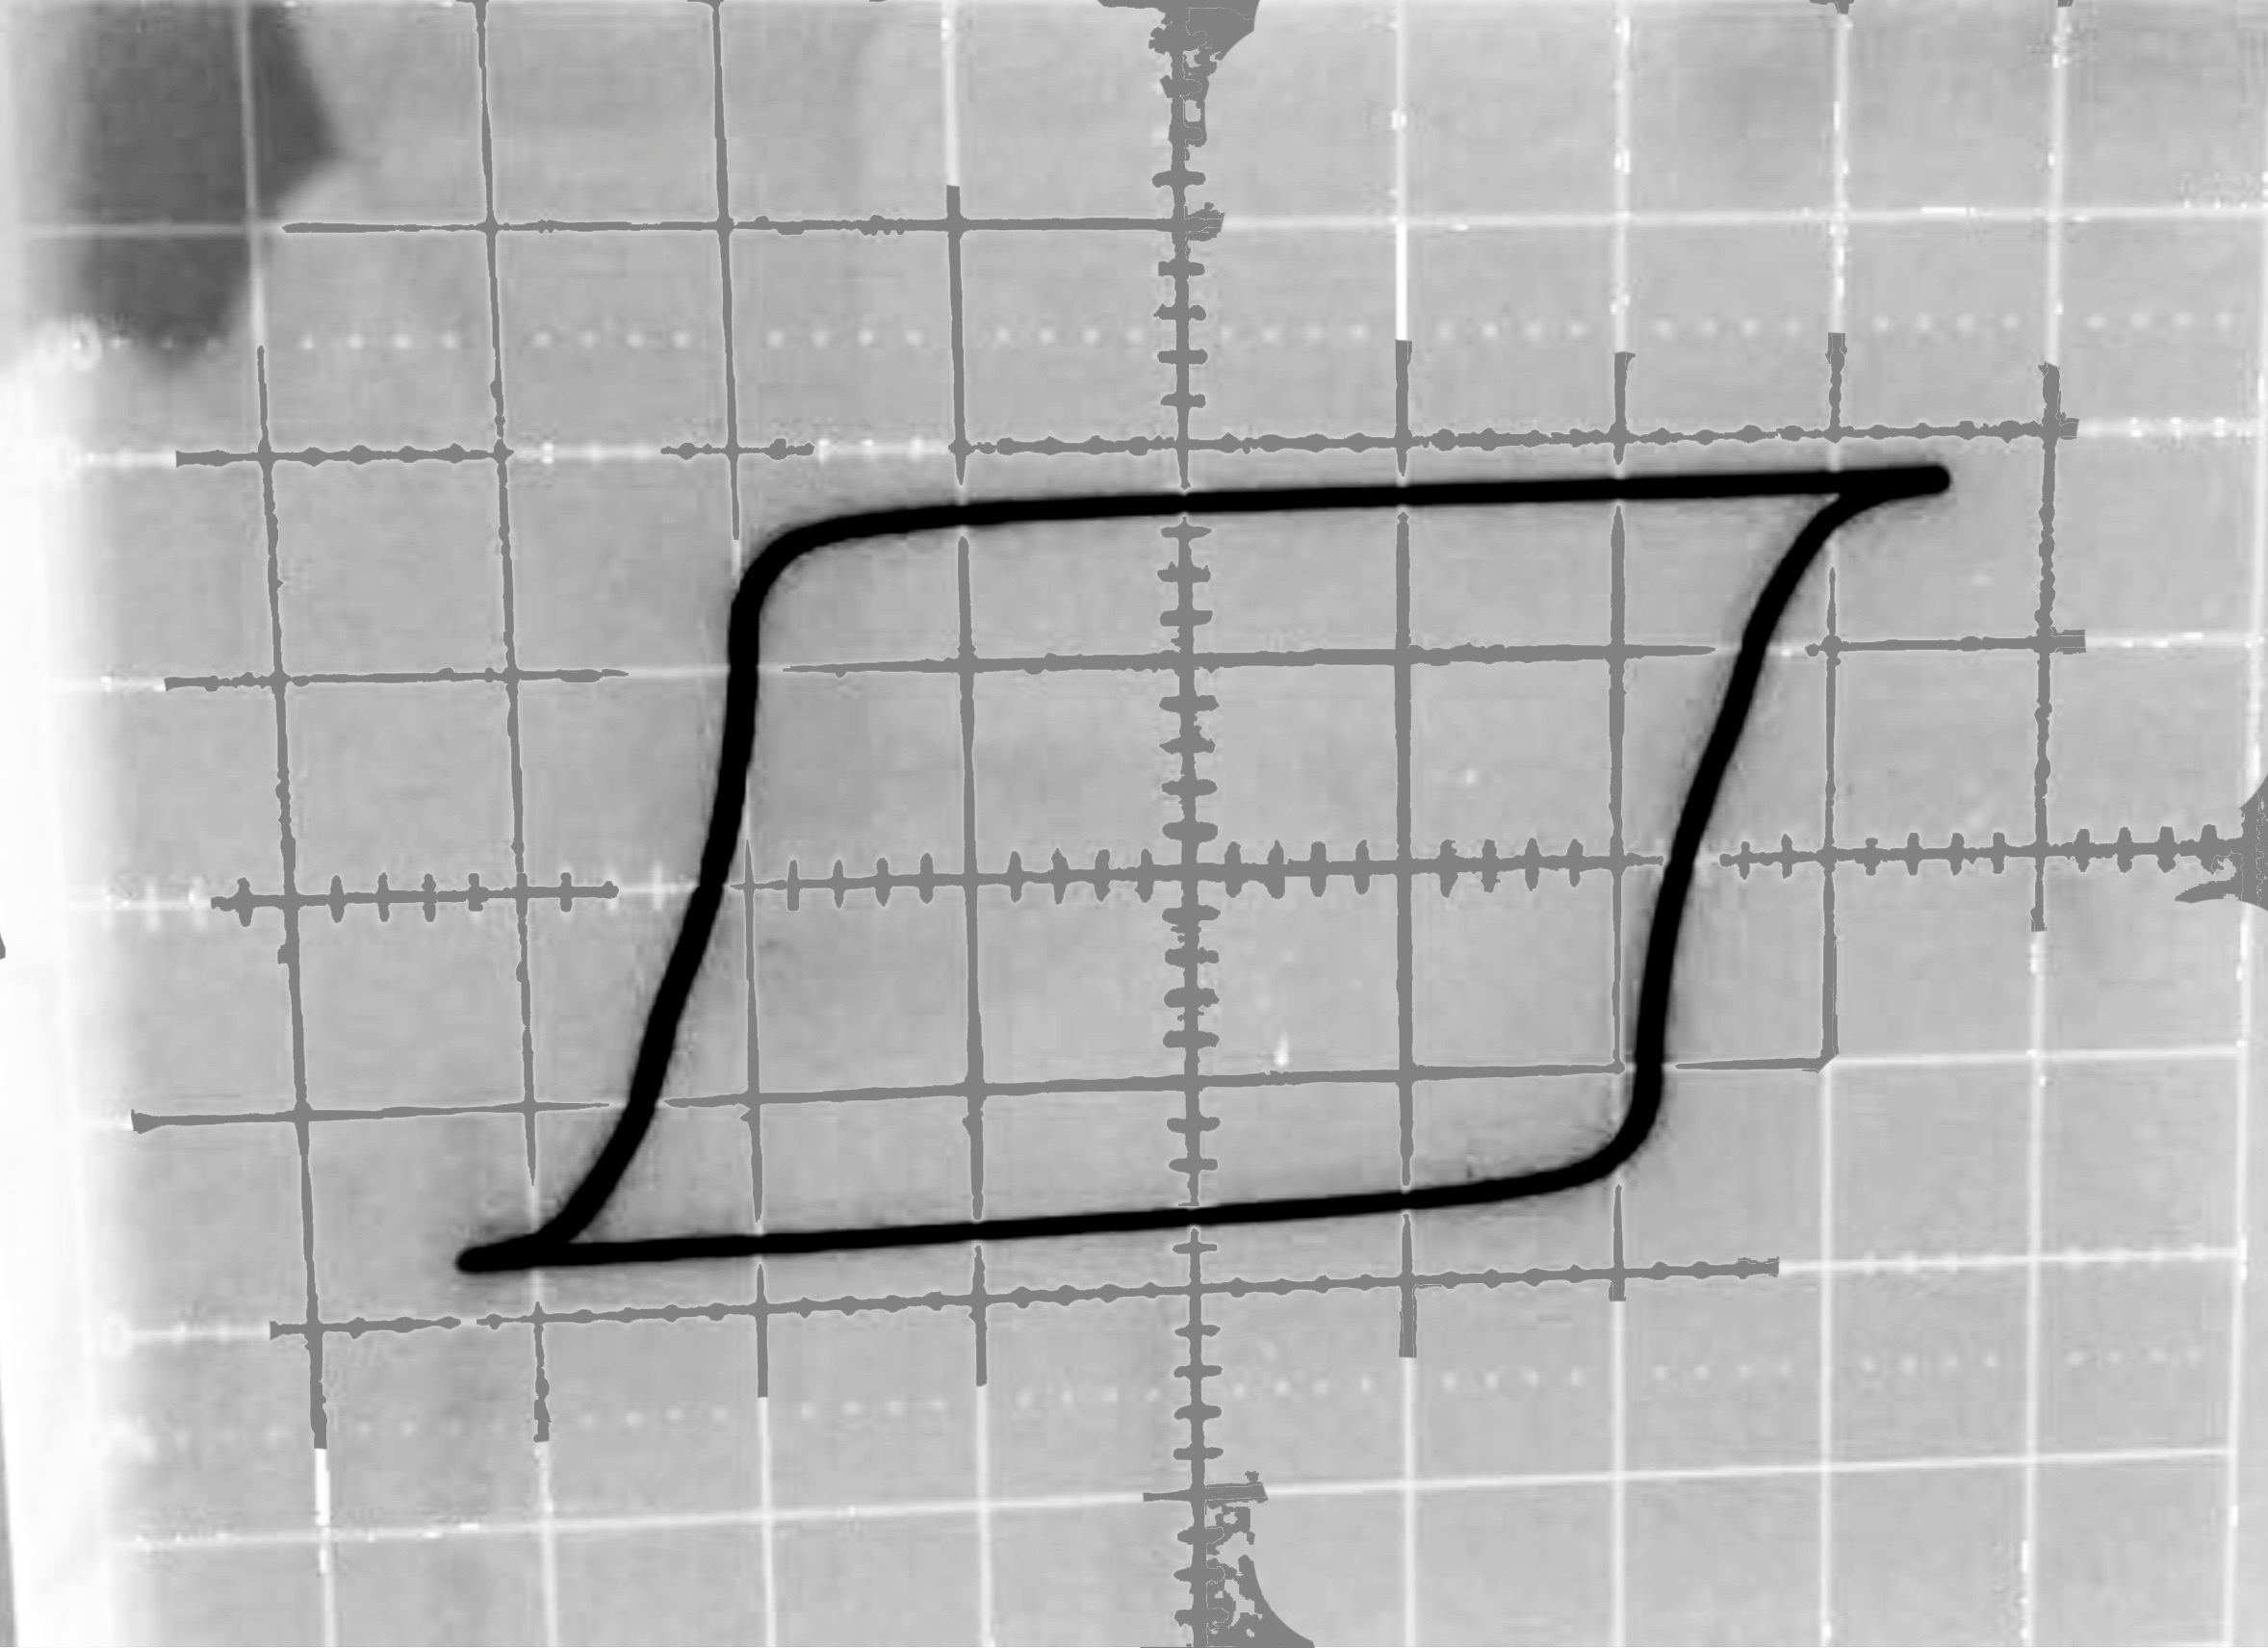
\includegraphics[scale=0.2]{2.png}
			      \caption{Петля гистерезиса для пермаллоя}
		      \end{figure}
		      \begin{table}[H]
			      \caption{Начальная кривая намагничивания для пермаллоя}
			      \begin{center}
				      \begin{tabular}{|c|c|c|c|c|c|c|c|c|c|c|c|c|c|}
					      \hline
					      №          & 1   & 2   & 3   & 4   & 5   & 6   & 7   & 8 \\ \hline
					      $ x $, дел & 14 & 13 & 12 & 11 & 10 & 9 & 8 & 7 \\
					      $ y $, дел & 8 & 7 & 7 & 7 & 6 & 4 & 1 & 0 \\
					      \hline
				      \end{tabular}
			      \end{center}
		      \end{table}

		      \begin{figure}[H]
			      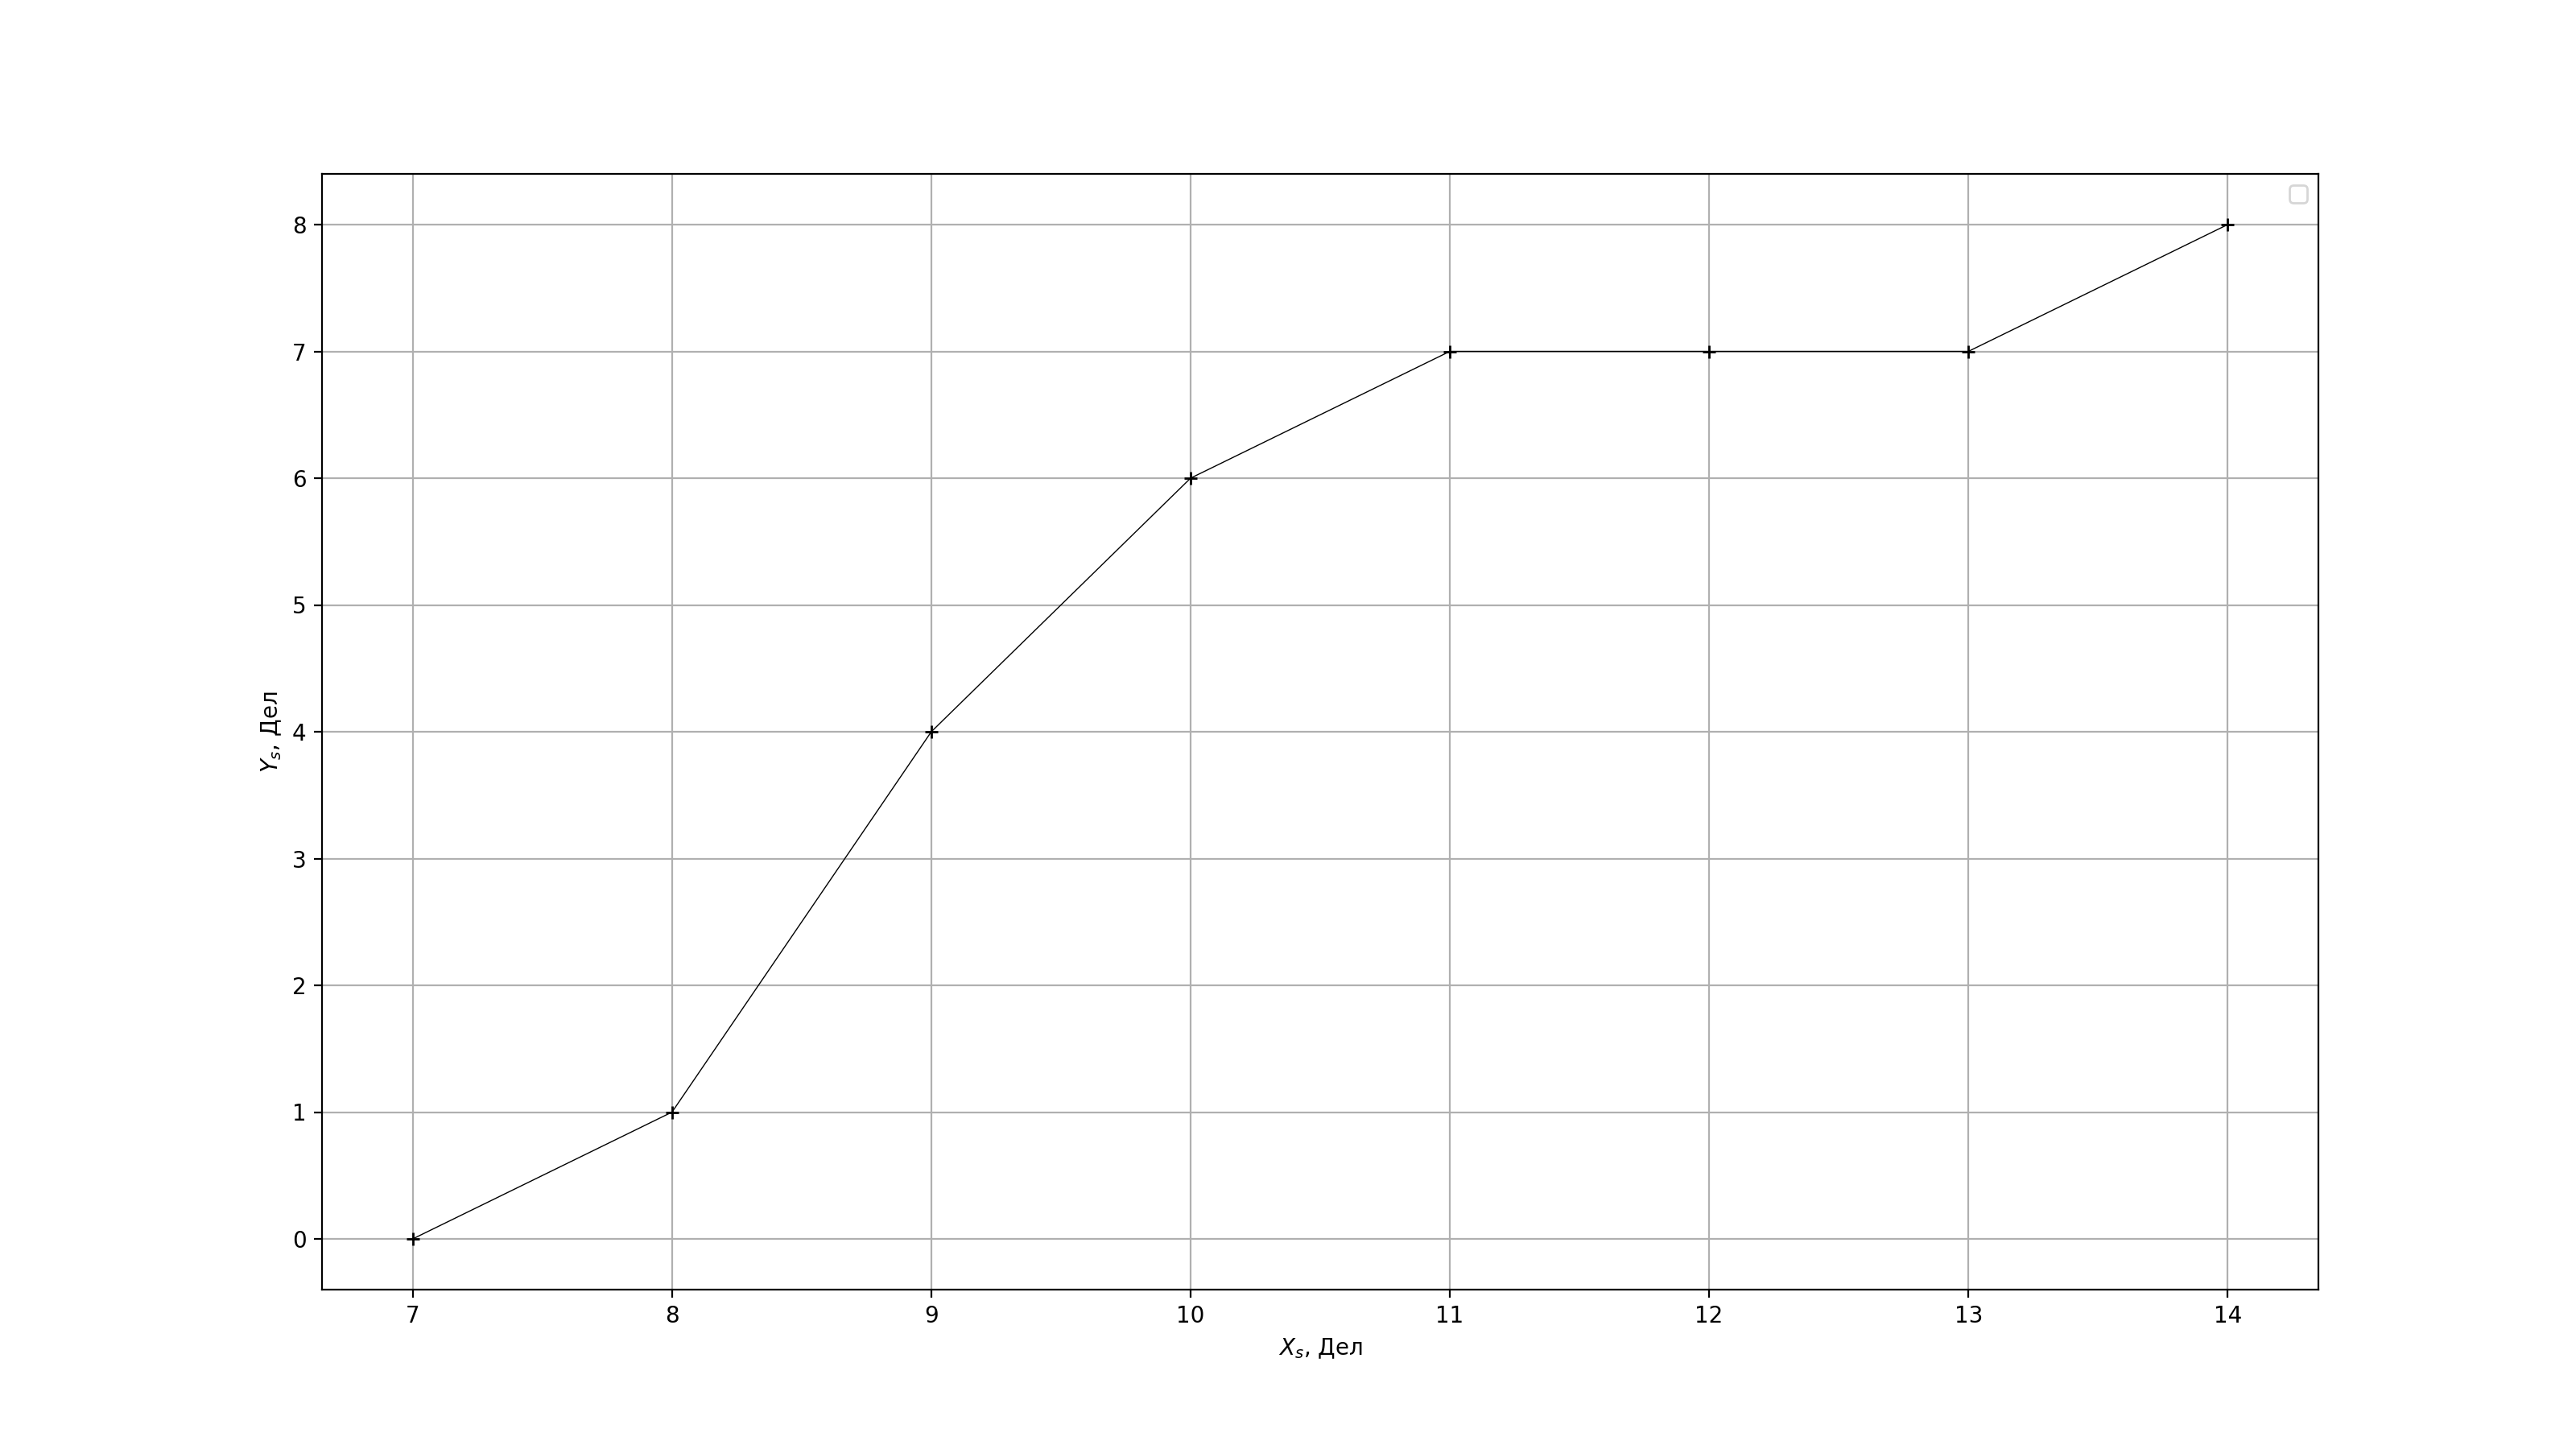
\includegraphics[scale=0.5]{graph1.png}
			      \caption{Начальная кривая намагничивания пермаллоя - график}
		      \end{figure}

			  \begin{figure}[H]
				  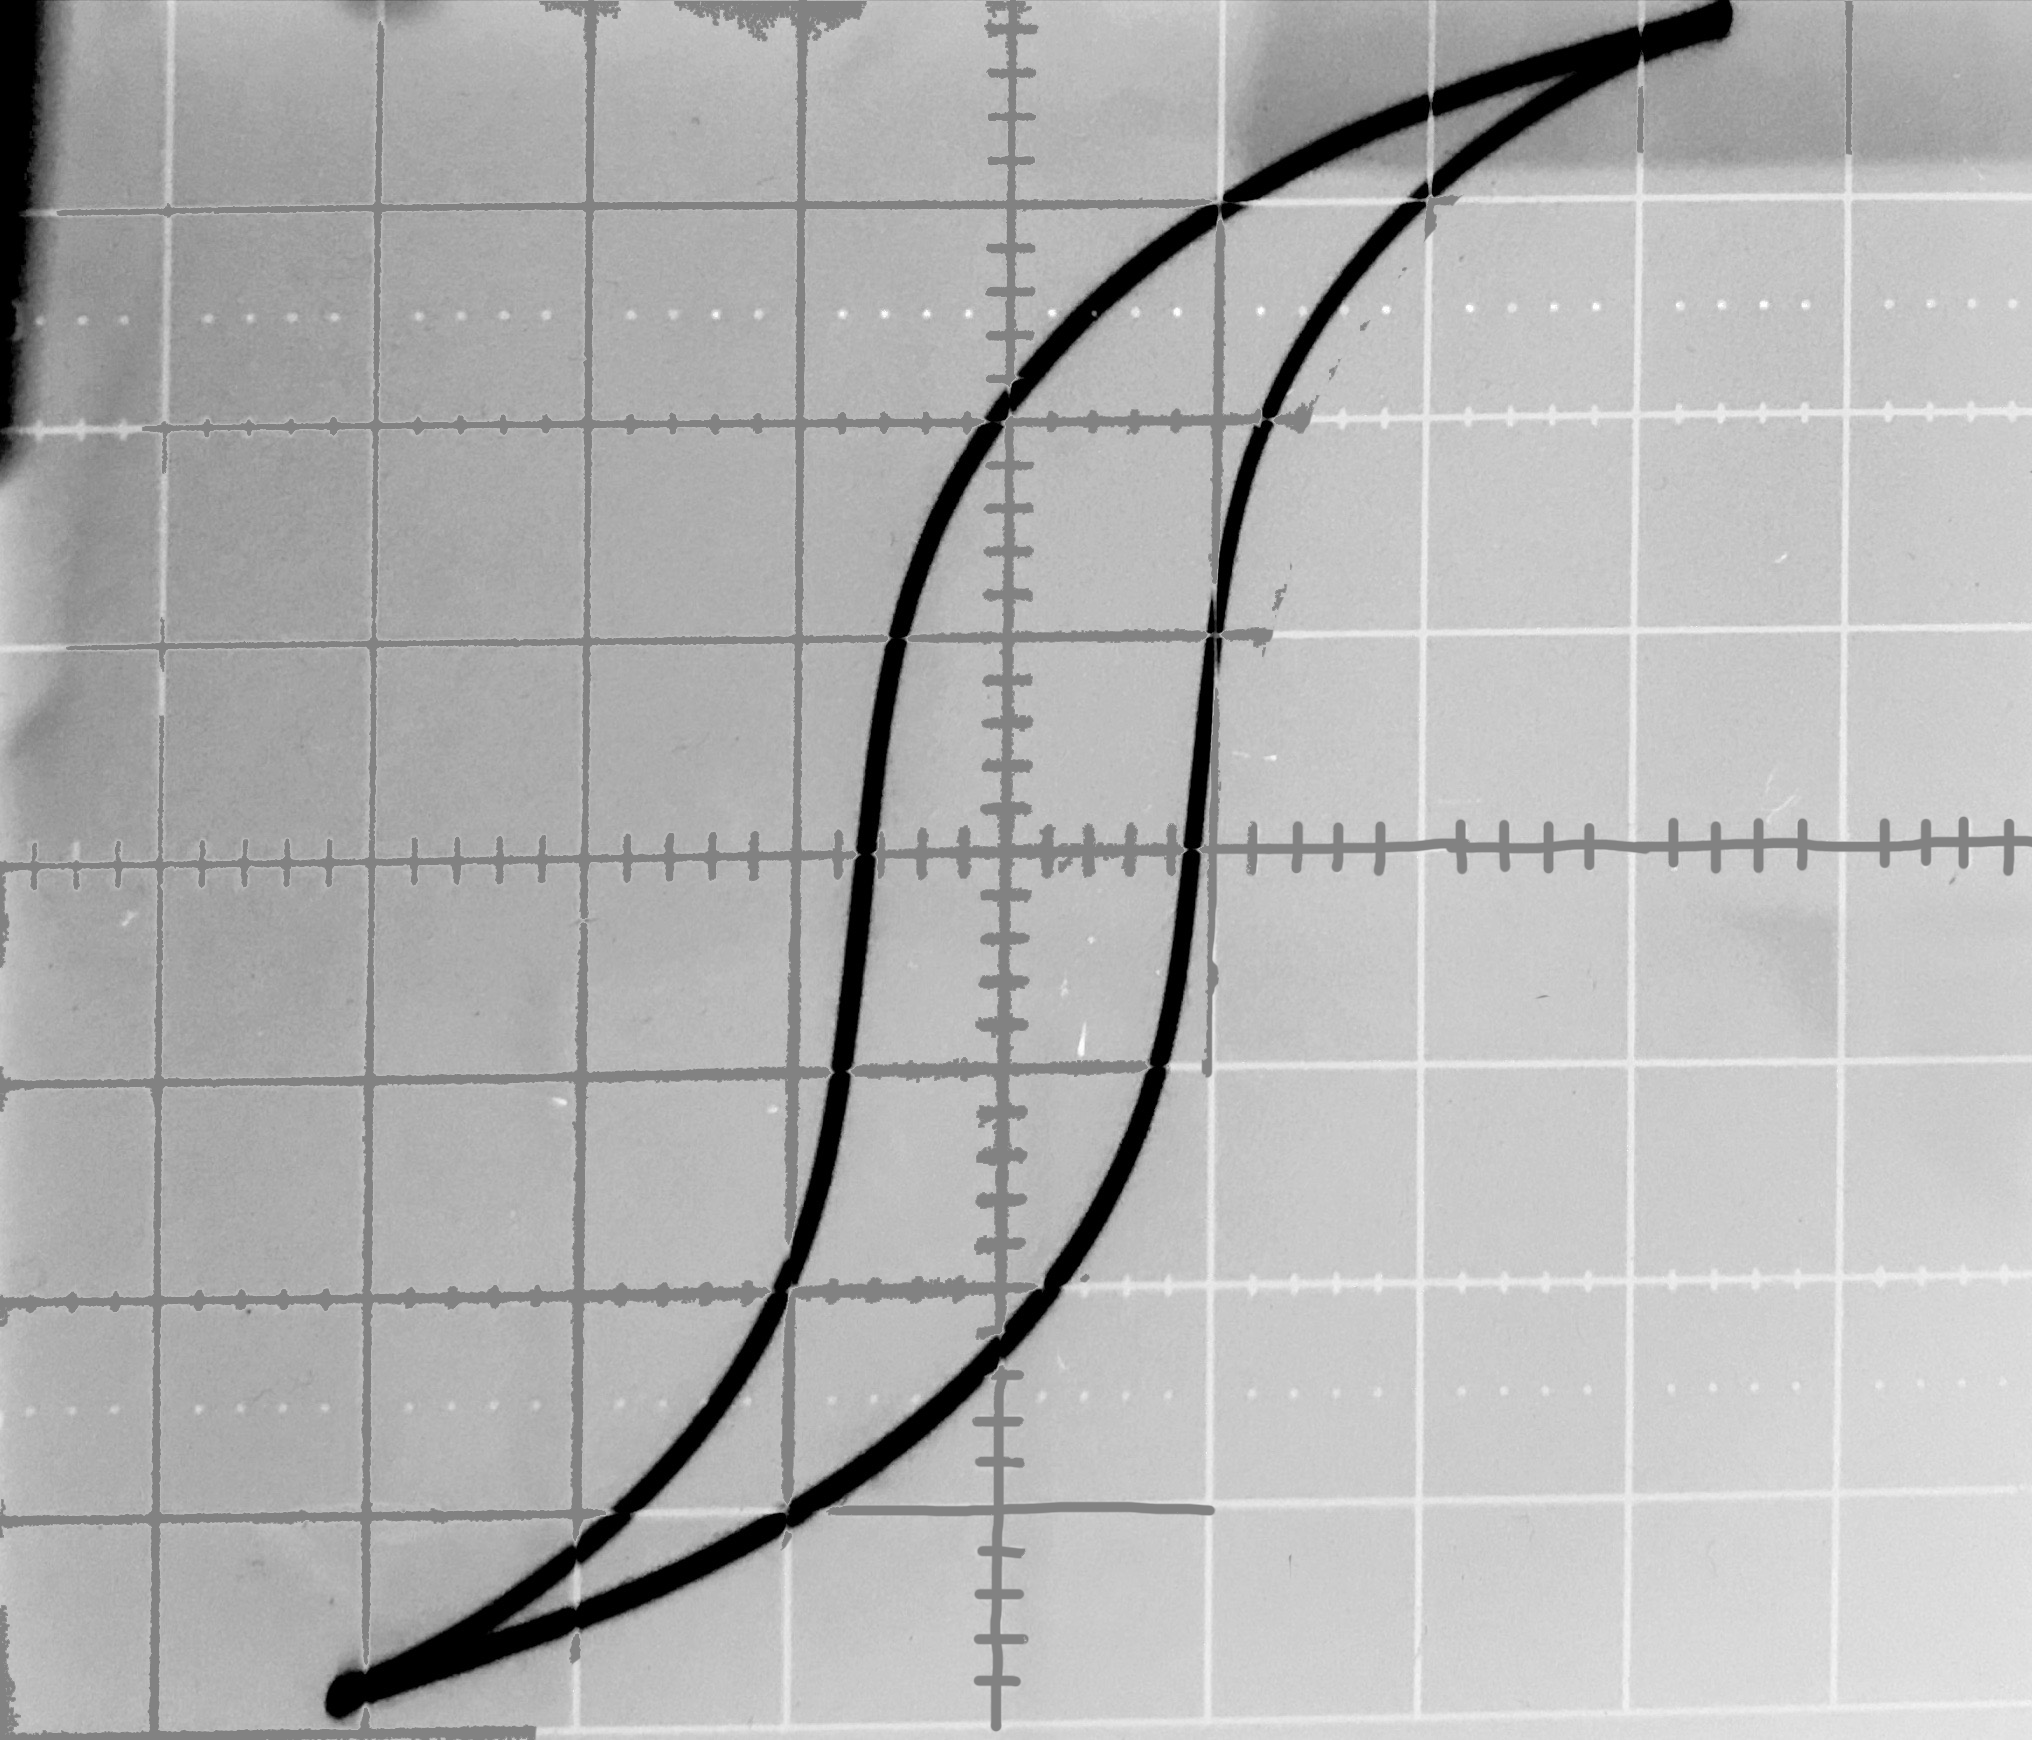
\includegraphics[scale=0.22]{3.png}
				  \caption{Петля гистерезиса для феррита}
			  \end{figure}

		      \begin{table}[H]
			      \caption{Начальная кривая намагничивания для феррита}
			      \begin{center}
				      \begin{tabular}{|c|c|c|c|c|c|c|c|c|c|c|c|c|c|}
					      \hline
					      №          & 1   & 2   & 3   & 4   & 5   & 6   & 7   & 8 \\ \hline
					      $ x $, дел & 9 & 8 & 7 & 7 & 6 & 6 & 5 & 4.5 \\
					      $ y $, дел & 10 & 8 & 7 & 6 & 5 & 3 & 3 & 2 \\
					      \hline
				      \end{tabular}
			      \end{center}
		      \end{table}

		      \begin{figure}[H]
				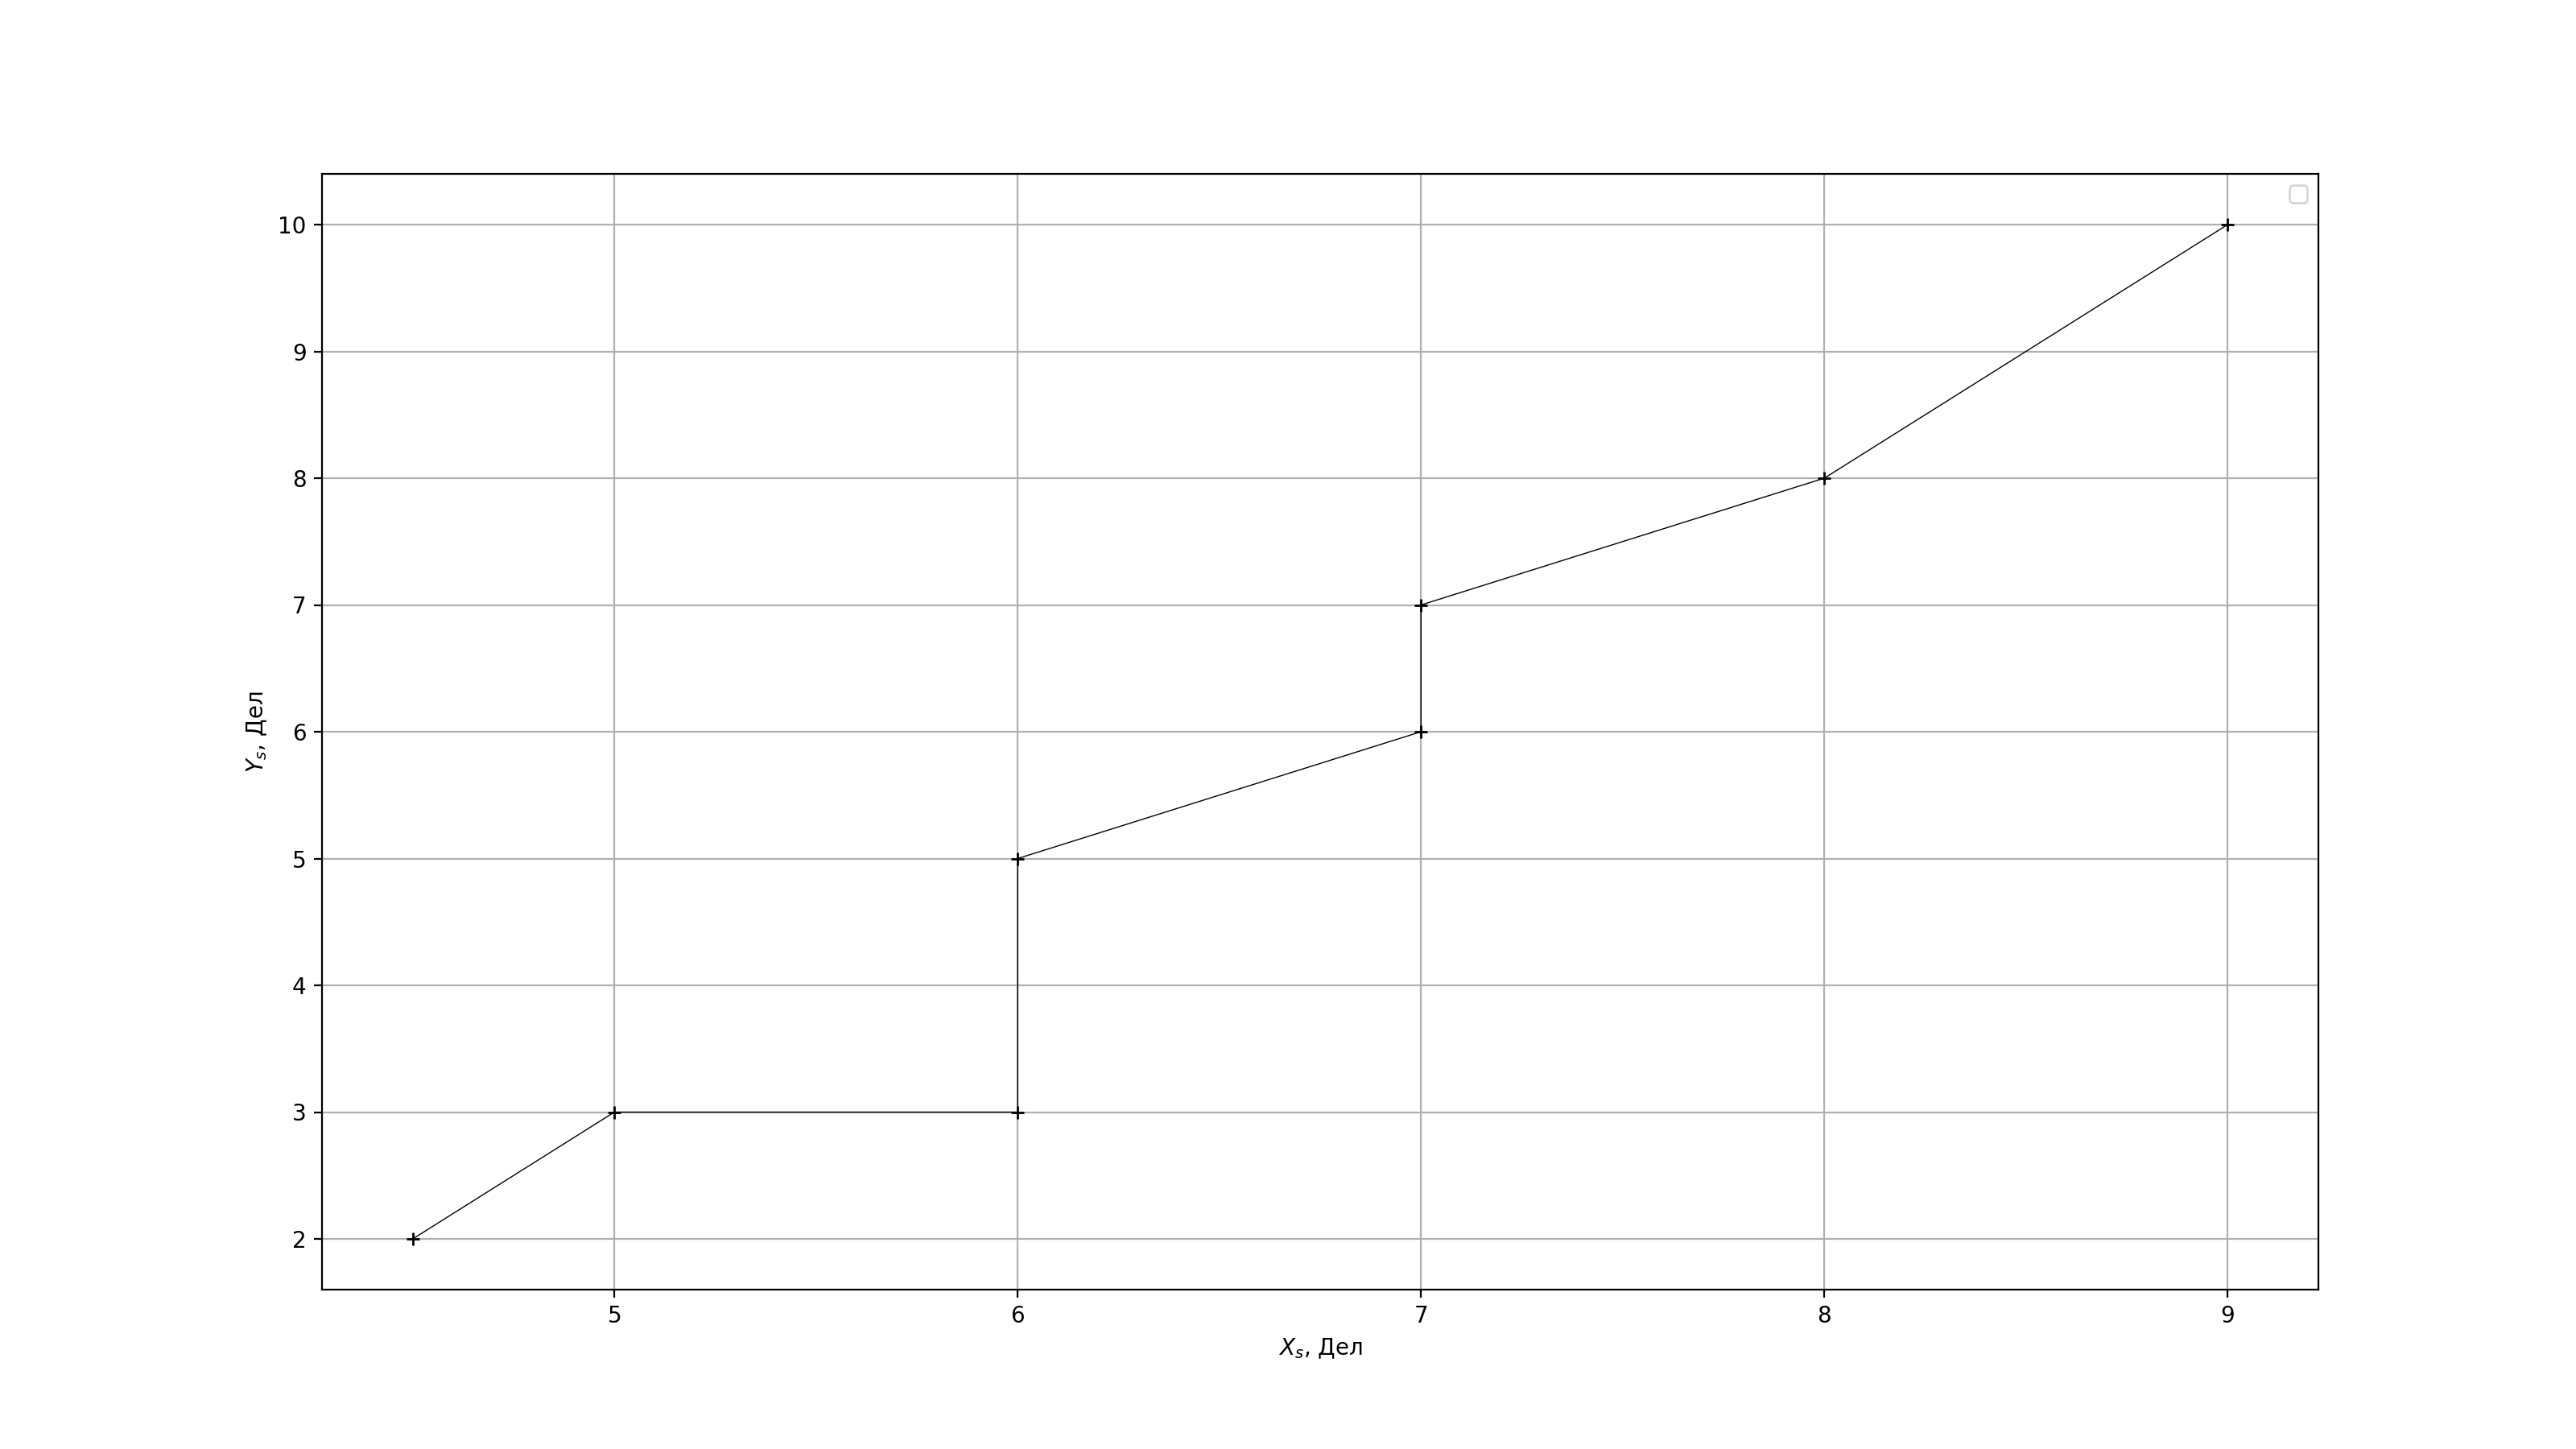
\includegraphics[scale=0.5]{graph2.png}
				\caption{Начальная кривая намагничивания феррита - график}
			  \end{figure}

			  \begin{figure}[H]
				  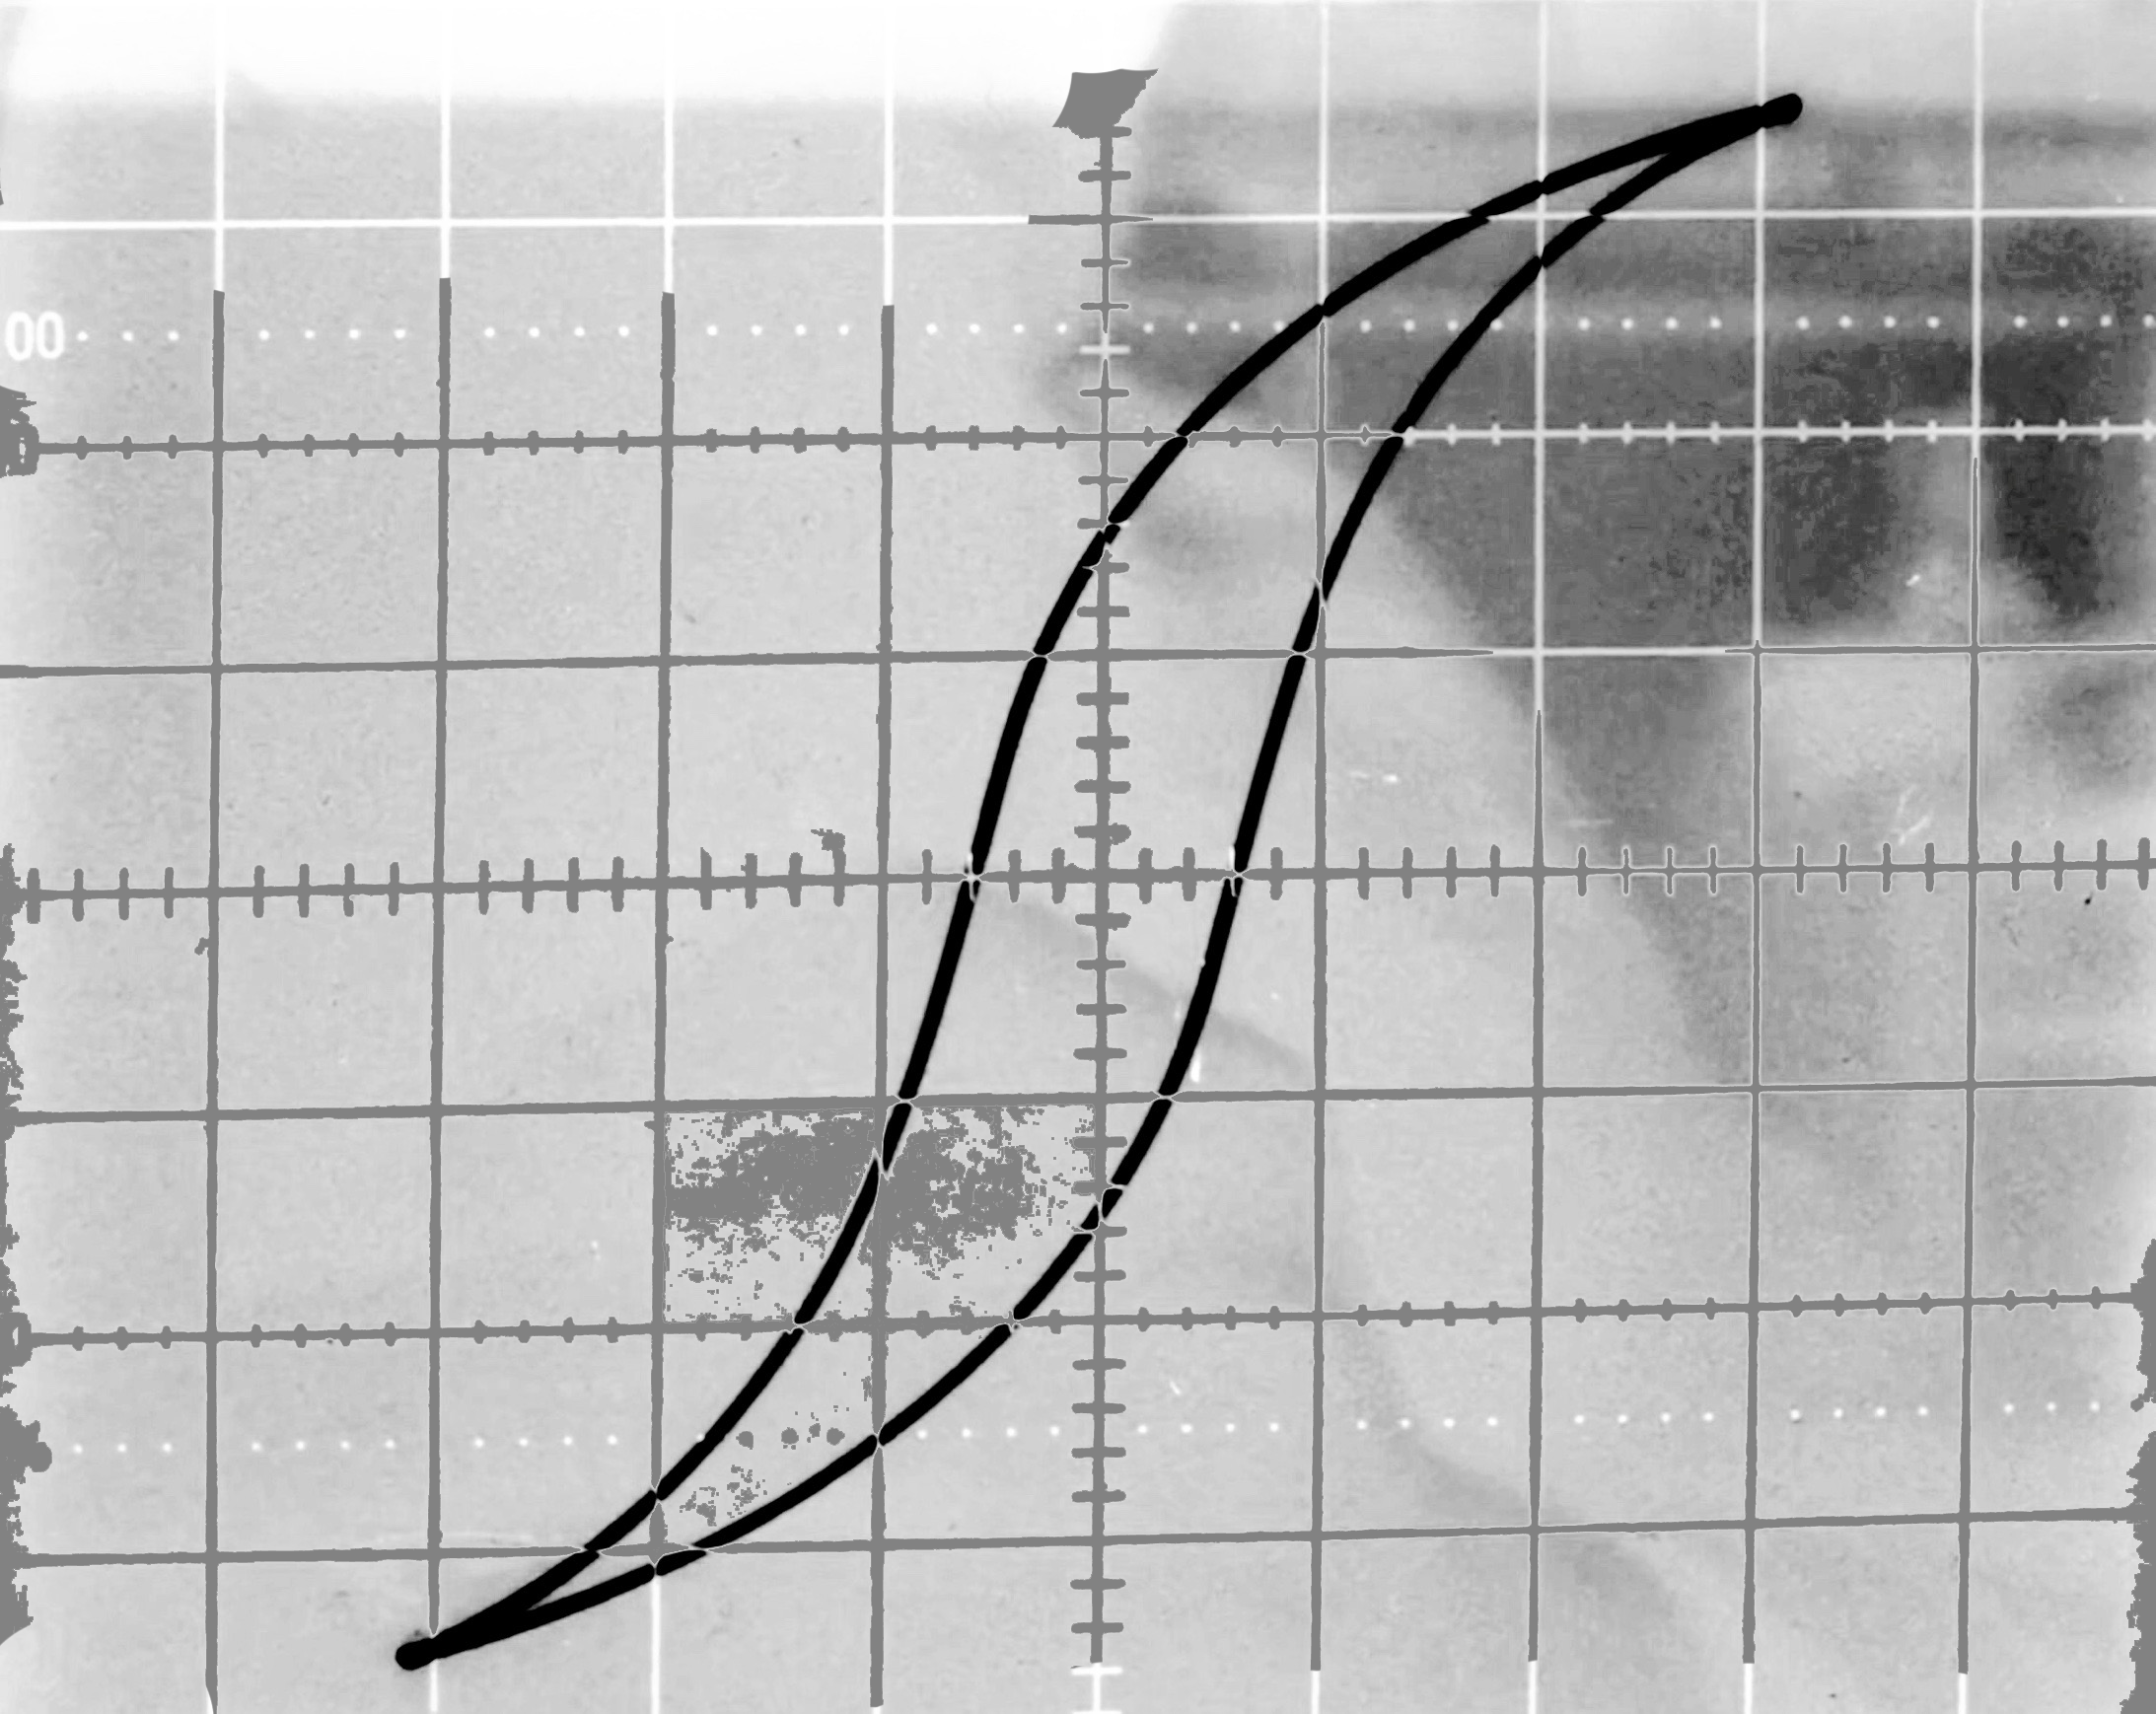
\includegraphics[scale=0.22]{1.png}
				  \caption{Петля гистерезиса для кремнистого железа}
			  \end{figure}

		      \begin{table}[H]
			      \caption{Начальная кривая намагничивания для кремнистого железа}
			      \begin{center}
				      \begin{tabular}{|c|c|c|c|c|c|c|c|c|c|c|c|c|c|c|c|c|c|}
					      \hline
					      №          & 1   & 2   & 3   & 4   & 5   & 6   & 7   & 8   & 9   & 10  & 11  & 12  & 13 & 14 & 15 & 16 \\ 	\hline

					      $ x $, дел & 20 & 19 & 18 & 17 & 16 & 15 & 14 & 13 & 12 & 11 & 10 & 8 & 6 & 4 & 2 & 1 \\
					      $ y $, дел & 14 & 14 & 14 & 13 & 13 & 13 & 12 & 12 & 11 & 11 & 10 & 8 & 7 & 4 & 1 & 0 \\
					      \hline
				      \end{tabular}
			      \end{center}
		      \end{table}

			  \begin{figure}[H]
				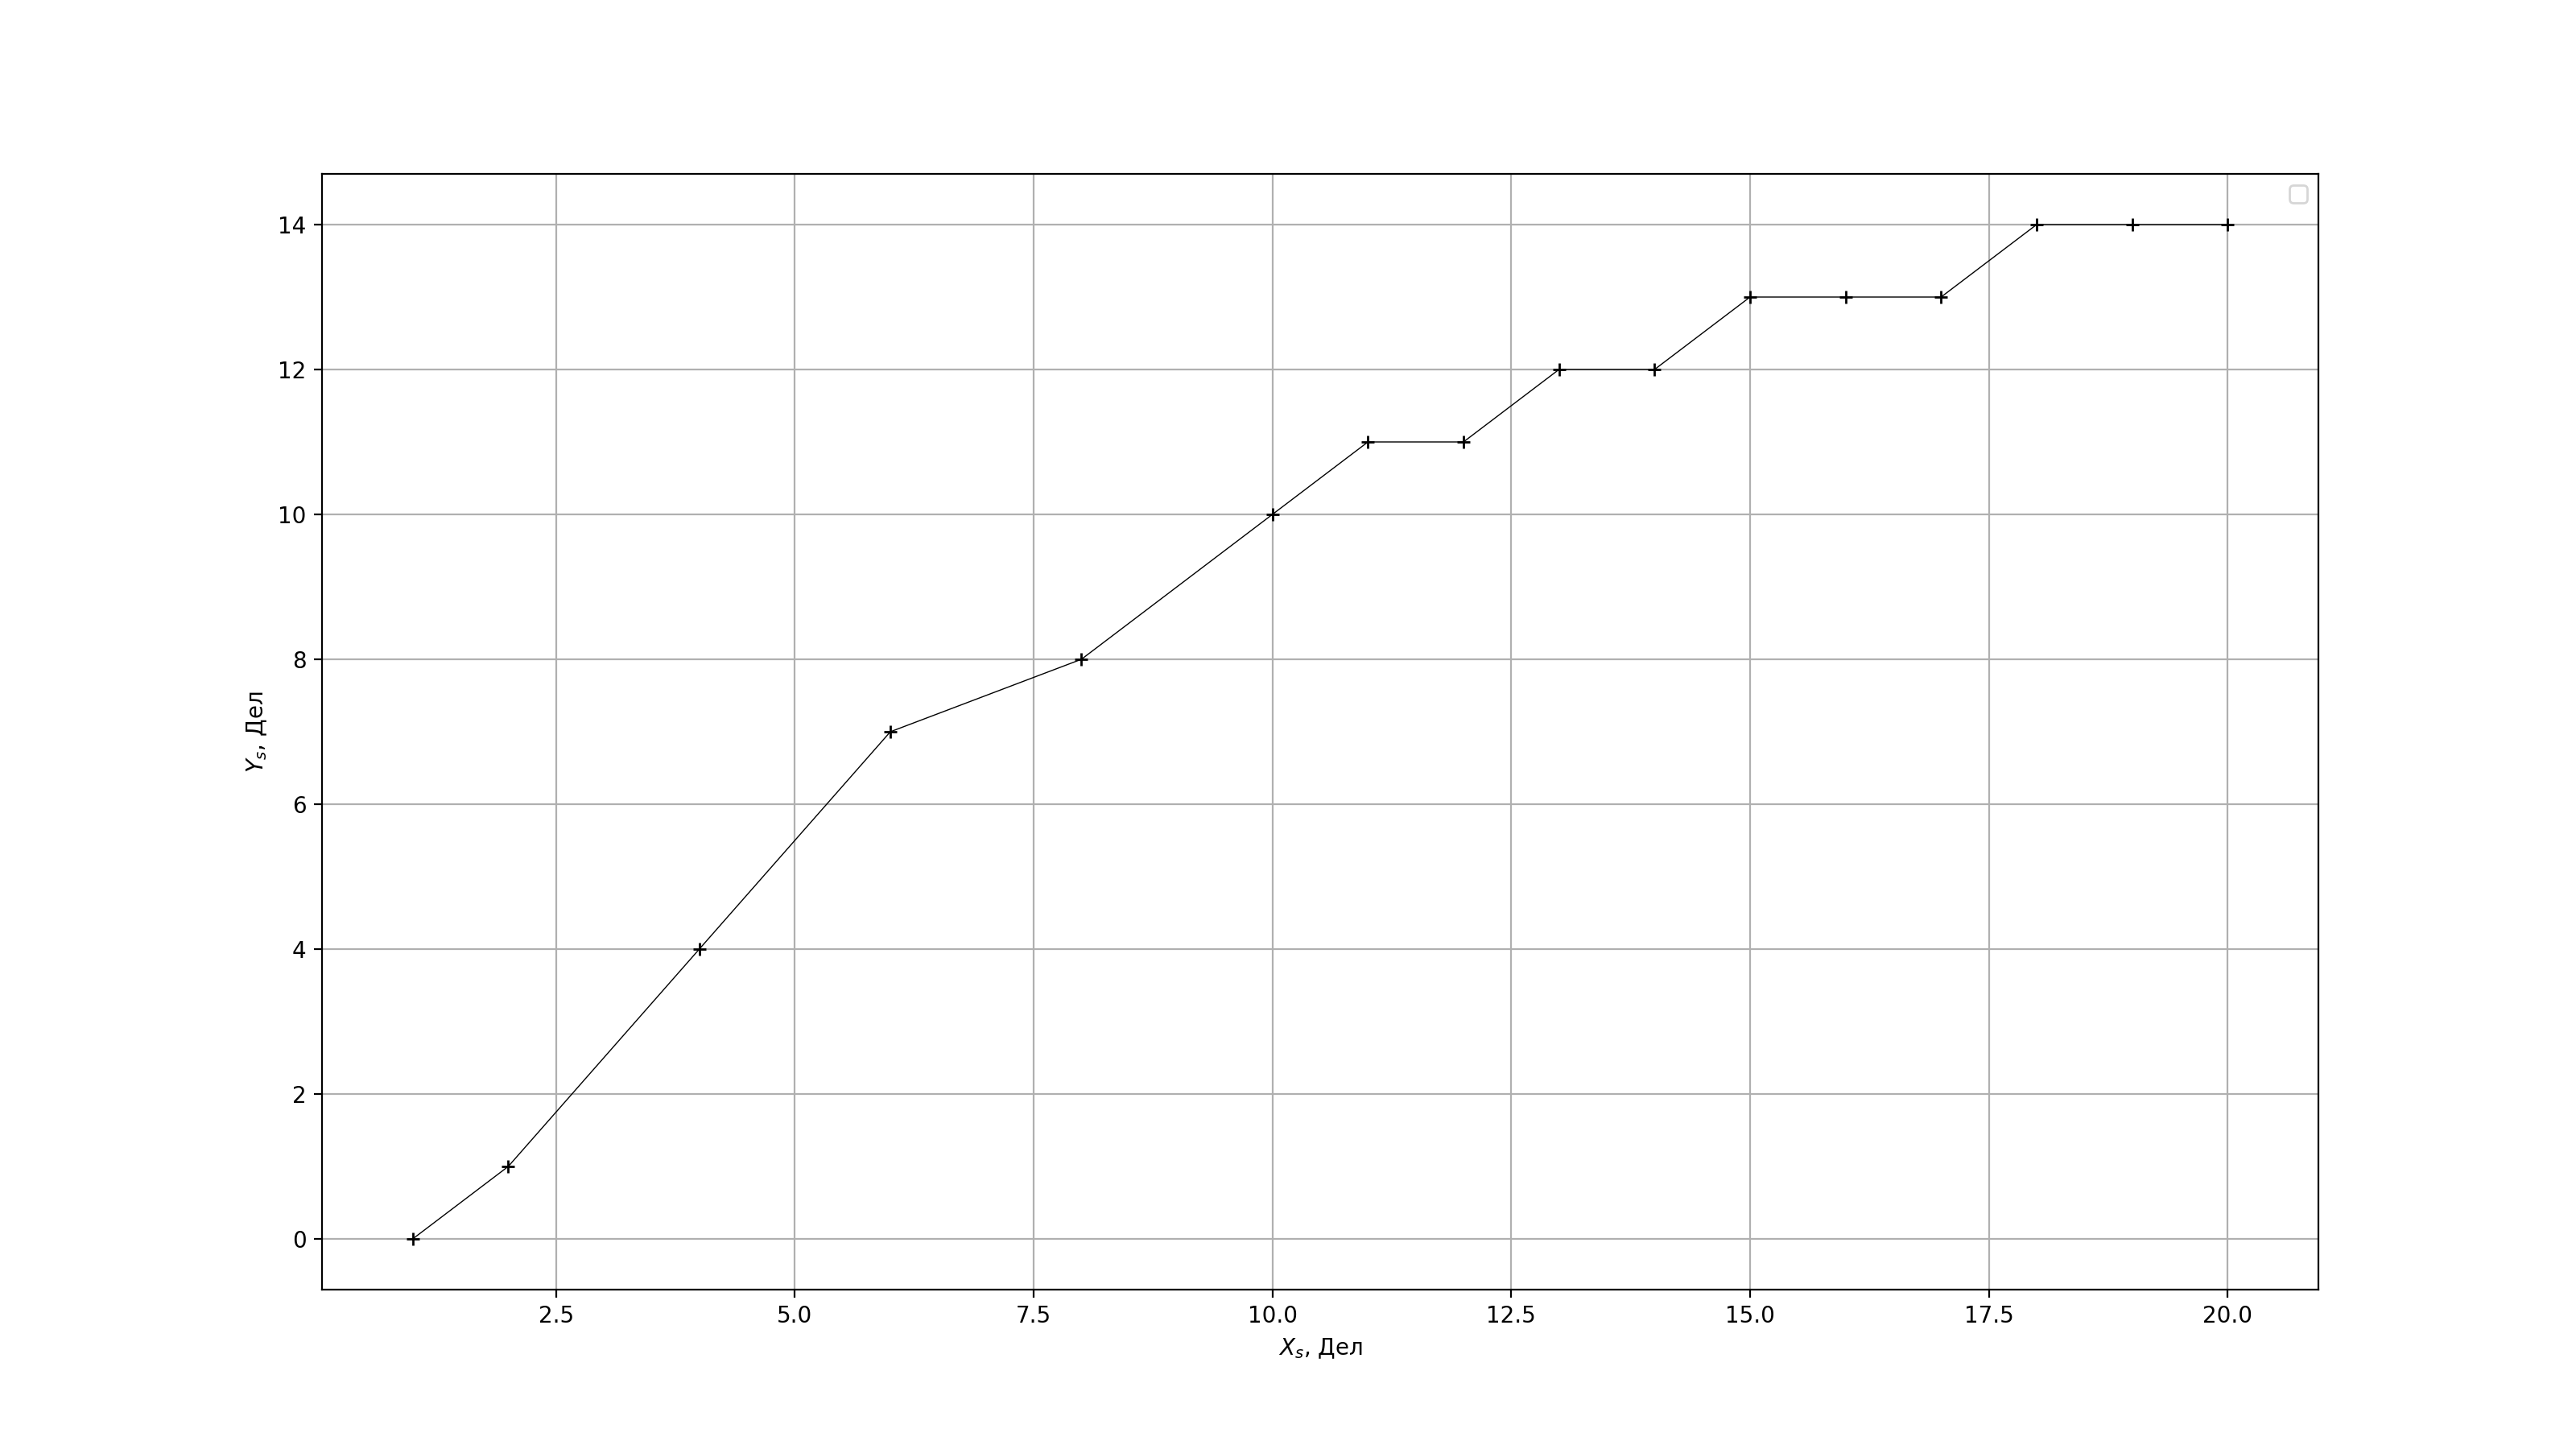
\includegraphics[scale=0.5]{graph3.png}
				\caption{Начальная кривая намагничивания феррита - график}
			  \end{figure}

	\item Восстановим предельные петли для образцов. Рассчитаем  цену деления ЭО для петли для оси Х (в $\dfrac{А}{м}$) по формуле

	      $$H=\dfrac{IN_{0}}{2\pi R},$$

	      где $I=\dfrac{K_{x}}{R_{0}}$, и в Теслах на деление для оси Y по формуле

	      $$B=\dfrac{R_\text{и} C_\text{и} U_\text{вых}}{SN_\text{и}},$$

	      где $U_\text{вых}=K_{y}.$


	      \begin{itemize}
			\item	\textbf{Пермаллой}:

			$H=0.022 \dfrac{\text{А}}{\text{м}}.$
			$B=0.1 \cdot 10^{-5}\dfrac{\text{Т}}{\text{дел}}.$


			\item	\textbf{Феррит}:

			$H=0.009 \dfrac{\text{А}}{\text{м}}.$
			$B=6.67 \cdot 10^{-7}\dfrac{\text{Т}}{\text{дел}}.$

			\item \textbf{Кремниевое железо}:

			$H=0.12 \dfrac{\text{А}}{\text{м}}.$
			$B=9.52 \cdot 10^{-6}\dfrac{\text{Т}}{\text{дел}}.$

	      \end{itemize}


	\item Соединим вход ячейки с обмоткой "<6,3 В"> трансформатора.

	      Определим входное напряжение на $ RC $-цепочке: $U_\text{вх}=2y\cdot K_{y} = 40$ В.

	      Не меняя тока, переключим Y-вход ЭО к выходу ячейки и аналогичным образом определим $U_\text{вых} = 0.3$ В.

	      Определим $\tau = RC $ по формуле

	      $$\tau = \dfrac{U_\text{вх}}{\Omega U_\text{вых}}=0.42 \pm 0.06 \; \text{Ом}\cdot \text{Ф}.$$

	      % Полученное значение $\tau \approx R_и C_и = 0,4 \; Ом \cdot Ф$.
	      Полученное значение $\tau \approx R_\text{и} \cdot C_\text{и} = 0.4 \; \text{Ом}\cdot \text{Ф}$

	\item Рассчитаем коэрцитивную силу $H_{c}$ и индукцию насыщения $B_{s}$ для каждого образца.

	      \begin{itemize}

			\item	\textbf{Пермаллой}:

			\fbox{$H_\text{c}=24.4 \pm 0.5 \dfrac{\text{А}}{\text{м}}$}\\
			\fbox{$B_{s}=1.82 \pm 0.06 \ \text{Тл}$}

			\item	\textbf{Феррит}:

			\fbox{$H_{c}=8.1 \pm 0.2 \dfrac{\text{А}}{\text{м}}$}\\
			\fbox{$B_{s}=(12.9\pm 0.02) \cdot 10^{-2} \text{Тл}$}

			\item 	\textbf{Кремниевое железо}:

				  \fbox{$H_{c}=54.5 \pm 0.8 \dfrac{\text{А}}{\text{м}}$}\\
				  \fbox{$B_{s}=0.70 \pm 0.03 \ \text{Тл}$}
		  \end{itemize}

	% \item Из графиков (4-6) оценим максимальные значения дифференциальной магнитной проницаемости.

	%       \begin{itemize}
	% 	      \item 	\textbf{Кремнистое железо}:

	% 	            \fbox{$\mu_{max} \simeq (30,6 \pm 2,9 ) \cdot 10^3 $}

	% 	      \item	\textbf{Пермаллой}:

	% 	            \fbox{$\mu_{max} \simeq (89,7 \pm 7,6) \cdot 10^3 $}

	% 	            \textbf{Феррит}:

	% 	      \item	\fbox{$\mu_{max} \simeq (7,6 \pm 0,6) \cdot 10^3$}

	    %   \end{itemize}

\end{enumerate}
\end{document}